\documentclass[runningheads,a4paper]{llncs}
\usepackage[utf8]{inputenc}
\usepackage{amssymb}
\setcounter{tocdepth}{3}
\usepackage{float}
\usepackage{caption}
\usepackage{graphicx}
\usepackage{subfigure}
\graphicspath{{images/}}

\usepackage[]{booktabs}
\usepackage{hyperref}
\hypersetup{
    colorlinks=true,
    linkcolor=blue,
    filecolor=magenta,      
    urlcolor=blue,
}

\usepackage{url}

\newcommand{\keywords}[1]{\par\addvspace\baselineskip
\noindent\keywordname\enspace\ignorespaces#1}

\makeatletter
\newcommand{\printfnsymbol}[1]{%
  \textsuperscript{\@fnsymbol{#1}}%
}
\makeatother

\begin{document}

\mainmatter  % start of an individual contribution

% first the title is needed
\title{Recognizing Handshapes using Small Datasets}

% a short form should be given in case it is too long for the running head
\titlerunning{Recognizing Handshapes using Small Datasets}


\author{Ulises Jeremias Cornejo Fandos \inst{1}\thanks{equal contribution}%
\and Gaston Gustavo Rios \inst{1, 3}\printfnsymbol{1} \and \\ Franco Ronchetti \inst{1} \and Facundo Quiroga \inst{1} \and Waldo Hasperué \inst{1,2} \and Laura Lanzarini  \inst{1}}
%
\authorrunning{Cornejo \and Rios \and Ronchetti \and Quiroga \and Hasperué \and Lanzarini al.}


\def\aa{\}}
\def\ab{\{}

\institute{
$^{1}$ Facultad de Informática, Universidad Nacional de La Plata \\
$^{2}$  Investigador Asociado - Comisión de Investigaciones Científicas (CIC) \\
$^{3}$  Becario de entrenamiento - Comisión de Investigaciones Científicas (CIC)
 \\ \email{\ab ucornejo,grios\aa @lidi.info.unlp.edu.ar}
}

\maketitle
\begin{abstract}
Advances in convolutional neural networks have  made possible significant  improvements in the state-of-the-art in image classification. However, their success on a particular field rests on the possibility of obtaining labeled data to train networks.  Handshape recognition from images,  an important subtask  of both gesture and sign language recognition,  suffers from such a lack of data.  Furthermore,  hands are highly deformable objects and therefore handshape classification  models require larger datasets.

We analyze both state-of-the-art models for image classification, as well as data augmentation schemes and specific models to tackle  problems with small datasets.  In particular,  we perform experiments with Wide-DenseNet, a state-of-the-art convolutional architecture and Prototypical Networks, a state-of-the-art few-shot learning meta model. In both cases, we also quantify the impact of data augmentation on accuracy. 

Our results show that on small and simple data sets such as CIARP,  all models and variations of achieve perfect accuracy,  and therefore the utility of the data is highly doubtful, despite its having 6000  samples. On the other hand, in small but complex datasets such as LSA16 (800 samples),  specialized methods such as Prototypical Networks do have an advantage over other methods.  On RWTH, another complex and small dataset with close to 4000 samples,  a  traditional and state-of-the-art method such as Wide-DenseNet surpasses  all other models.  Also, data augmentation consistently increases accuracy for Wide-DenseNet,  but not full  Prototypical Networks.

\keywords{ sign language, hand shape recognition,convolutional neural networks,densenet,  prototypical networks, small datasets}
\end{abstract}

        

\section{Introduction}


Hand shape recognition is a crucial component of any sign language recognition system. In recent years, new advances in machine learning   using models such as  convolutional neural networks  and recurrent neural s have improved our ability to tackle complex Recognition problems such as speech recognition. However, sign language recognition has not  been able to take advantage of most of these advances, since  the availability of labeled, quality data for training models is currently very limited \cite{}.   

In this article we propose to  employ and compare new methods devoted to deal with small and unlabeled data sets in order to improve the current state-of-the-art in hand shape recognition for sign language. 

our approach consists of combining and comparing three different techniques For improving model performance in these conditions: data augmentation,  prototipical learning and semi supervised learning.
for data augmentation we employ several... We combine datasets X and Y ...
We also employ prototypical networks to
matching Networks are a recent technique developed to take advantage of and label data.  we apply matching Networks to the rwth dataset.

\section{Datasets and Models}
\label{sec:datasetsmodels}
We selected three datasets, LSA16 \cite{Ronchetti2016}, RWTH-PHOENIX-Weather (RWTH) \cite{koller16:deephand} and CIARP \cite{ciarp2018},  because they contain images whose setting varies greatly, have been evaluated already, and posses different quantities of examples or distributions of samples per class. 

We employed two different classification models to analyze their ability to learn from these small handshape datasets; Prototypical Networks \cite{protonet} and DenseNet \cite{densenet}. Prototypical Networks is a model that was designed explicitly to deal with small sample sizes. On the other hand, DenseNet is currently the state of the art  in image classification with convolutional neural networks, and while it has not been explicitly designed for small datasets, it has shown exceptional performance in many different tasks.

We also experimented with data augmentation to analyze its capacity to compensate for the lack of data.

In the following subsections we describe in more detail the selected datasets and models.

\subsection{Datasets}
\label{sec:datasets}

\subsubsection{LSA16}

This dataset contains images of 16 handshapes of the Argentinian Sign Language (LSA), each performed 5 times by 10 different subjects, for a total of 800 images. The subjects wore color hand gloves and dark clothes.

\subsubsection{RWTH}

This dataset is composed of a selection of images taken from the sign language interpreter at the German public tv-station PHOENIX. There are a total of 45 different hand signs. The interpreters wore dark clothes in front of an artificial grey background. 


\subsubsection{CIARP}

This dataset contains 6000 images with size of 38x38 acquired by a single color camera. The images were manually labeled and fit 10 classes of hand gestures. 

% TODO add reference to this figure in each datasets subsection
\begin{figure}
    \centering
    % \includegraphics{}
    \caption{Sample images from the LSA16 (first row), RWTH (second row) and CIARP (third row) datasets.}
    \label{fig:datasets}
\end{figure}

\subsection{Models}
\label{sec:models}
\subsection{Prototypical Networks for Small Datasets}
\label{models:protonet}

Prototypical Networks \cite{protonet} is a meta-learning model for the problem of few-shot classification, where a classifier must generalize to new classes not seen in the training set, given only a small number of examples of each new class. The ability of a algorithm to perform few-shot learning is typically measured by its performance on n-shot, k-way classification tasks. First a model is given a query sample belonging to a new, previously unseen class. Then, it’s also given a support set, S, consisting of n examples, each from k different unseen classes. Finally, the algorithm then has to determine which of the support set classes the query samples belong to.
Schemes for few shot classification tasks like Prototypical Networks can also be of use for training small datasets where all classes are known.

Prototypical Networks applies a compelling inductive bias in the form of class prototypes to achieve impressive few-shot performance. The key assumption is made is that there exists an embedding in which samples from each class cluster around a single prototypical representation which is simply the mean of the individual samples. This idea streamlines n-shot classification in the case of $n > 1$ as classification is simply performed by taking the label of the closest class prototype.

\subsection{DenseNet}

As our state of the art model we selected DenseNet because it can handle small datasets with low error rate\cite{pmlr-v80-pham18a}.

DenseNet \cite{densenet} works by concatenating the feature-maps of a convolutional block to the feature-maps of all the previous convolutional blocks and using this value as input for the next convolutional block. This way each convolutional block receives all the collective knowledge of the previous layers maintaining the global state of the network which can be accessed.

Convolutional networks construct informative features by fusion both spatial and chanel-wise information within local receptive fields at each layer. Squeeze and excitation blocks (SE block) \cite{Hu2017SqueezeandExcitationN} focus on the chanel-wise information used in the convolutional layers. SE blocks improve the quality of representations produced by the network by modeling the interdependency between channels to perform feature recalibration. SE blocks can be included in any model that uses convolutional layers to improve its performance at low computational cost. We added SE blocks to our DenseNet model to improve its performance.

\subsection{Data Augmentation}

Image data augmentation is a set of techniques that aim at artificially augmenting the amount of data that can be obtained from the images in the dataset. These techniques modify the images in the dataset  with a set of predefined operations to create new images that can be used to train a model.  In this manner, we can compensate  for the lack of  variability in a small dataset\cite{cubuk2019autoaugment}.


\section{Experiments}
\label{sec:experiments}
We performed classification experiments on LSA16, RWTH and CIARP  handshape datasets. For each experiment, we split the dataset in training and test sets, with the latter taking 25\% of the samples.  The split was stratified,  maintaining the proportion of samples of each class in both sets.

We applied normalization feature-wise substracting the mean and dividing by the standard deviation of each feature. For data augmentation we used horizontal flipping, a 10 and 30 degree rotation and a resampling of the images creating new versions of them with a different size reducing each image by 10\% and 20\% in width and height. We found that a 10 degree rotation gave better results because a rotation of 30 degrees showed to be too high for the nature of the datasets.

We made multiple experiments with Prototypical Networks and DenseNet to find out which hyperparameter configuration was the best for each dataset: with and without data augmentation. We describe the hyper parameters for each model/dataset combination.

\subsection{Prototypical Network}

As mentioned in section \ref{models:protonet}, we can use Prototypical Networks' ability to work with small datasets even if all samples are labeled.

Therefor we experimented with Prototypical Networks using an embedding architecture composed of four convolutional blocks. Each block comprises a \{64, 128\}-filter $3 x 3$ convolution, batch normalization layer, a ReLU nonlinearity and a $2 x 2$ max-pooling layer.

We used the same encoder for embedding both support and query points. All of our models were trained  with the ADAM\cite{Adam} optimizer. We used an initial learning rate of $10^{-3}$ and cut the learning rate in half every 2000 episodes.

We trained prototypical networks using Euclidean distance in the 1-shot and 5-shot scenarios with training episodes containing 16, 20 and 10 classes (for LSA16, RWTH and CIARP respectively) and 5 query points per class. We found it advantageous to match the same value of n for train and test scenarios, and to use a higher value of k (more classes) per training episode. We computed classification accuracy for our models by averaging over 1000 randomly generated episodes from the test set.

In the experiments performed with RWTH we used the same four-block embedding architecture by adding an eight-block architecture with the same layer composition with the idea of analyzing the need to increase the size of the network given the difficulty of the dataset. The difference in the results obtained in 1-shot and 5-shot scenarios for this dataset was very large. We found that 5-shot scenarios gave better results. Using this discovery we only used 5-shot learning in the remaining experiments.

The best configurations for all datasets is the 5-shot scenario with equals n for train and test scenarios by using more than or equal to 5 classes per training episode. Better results were obtained when the number of classes approaches the total amount of classes in the dataset except on CIARP where the best results were obtained when the number of classes per training episode is 5. In addition, the best configurations of the embedding architecture is a 64-filter for all datasets.

\subsection{Wide-DenseNet}

We employed a variation on DenseNet called Wide-DenseNet which follows the strategy used by wide residual networks.\cite{He2015DeepRL}.

We employed a Wide-DenseNet including SE blocks after each dense and transition block. We performed a grid search of hyperparameters to find the model with the best accuracy, averaged over all datasets. We tried growth rate values of 32, 64 and 128 and depth of dense layers of no more than [6,12,24,16], where each number represents the number of dense blocks.

We trained the models using a batch size of 16, an initial learning rate of $10^{-3}$ with categorical cross entropy optimizer and 400 epochs with a maximum patience of 25. The resulting model used a growth rate of 64 and two dense blocks with 6 and 12 layers respectively,  for all datasets.

\subsection{Results}

In table \ref{tab:results}, we can observe that all models have a lower accuracy on the RWTH dataset, which is expected since it has more classes, unsegmented hand images and class imbalances. Prototypical Networks have similar accuracy for LSA16 and CIARP datasets beating the rest of the models, also expected since both datasets have very few examples. For LSA16 they achieve better accuracy than VGG16 and DenseNet; and for CIARP they achieve similar or better accuracy than LeNet CNN and DenseNet. The accuracy of DenseNet on the RWTH is slightly bigger than for other models. Our hypothesis was that Prototypical Networks obtained low accuracy because the images of the hands were unsegmented. It should be noted that the use of data augmentation did not bring significant improvements in the accuracy obtained in LSA16 and CIARP.

Another fact to consider is that better results were obtained with those parameters that reduced the size of the architectures.

\begin{table}[h!]
\centering
\begin{tabular}{ p{17em} p{6em} p{6em} p{6em}}
\toprule
\emph{Method} & \emph{LSA16} &  \emph{RWTH}  &  \emph{CIARP} \\ \midrule
LeNet \cite{ciarp2018} & - & - & 99.20  \\
Inception (fine-tuning) \cite{koller16} & - & 85.50 \\
VGG16 \cite{quiroga2017study} & 95.92 & 82.88 \\
Inception+SVM (pre-trained) \cite{quiroga2017study} &  93.67 & 78.12 & - \\
DenseNet  & 98.07 & 91.10 & 99.93 \\
DenseNet ++  & 98.90 & \textbf{94.00} & 99.99 \\
Prototypical Networks  & 99.15 & 79.93 & 99.98 \\
Prototypical Networks ++ & \textbf{99.26} & 80.85 & \textbf{100.00} \\
\bottomrule
\end{tabular}
\caption{Accuracy of various convolutional neural network based models on three datasets: LSA16, RWTH and CIARP. Models with "++" used data augmentation as described in this section. \label{tab:results}}
\end{table}

In figure \ref{fig:results_varying_samples}, we can observe the accuracy of Prototypical Networks and DenseNet models trained by varying sample sizes. We performed experiments using the same embedding architectures and configurations described in this section varying the training sample sizes with percentages of 44\%, 67\% and 85\% and a fixed test size of 25\%. From the obtained results, we can see that the performance of the DenseNet models increases as more training examples are provided. From figure \ref{fig:results_varying_samples_rwth} we can see that the DenseNet model trained using data augmentation obtains better results than the one trained without. On the other hand, Prototypical Networks models do not show a significant increase in performance as the percentage of samples increases. In figures \ref{fig:results_varying_samples_rwth} and \ref{fig:results_varying_samples_ciarp} we can observe how the use of data augmentation, on RWTH and CIARP datasets respectively, results in Prototypical Networks models with great accuracy improvement compared to the results obtained on LSA16, figure \ref{fig:results_varying_samples_lsa16}), where the increase of performance from the use of data augmentation is minimal.

\begin{figure}[h]
\begin{tabular}{ccc}
    \subfigure[LSA16]{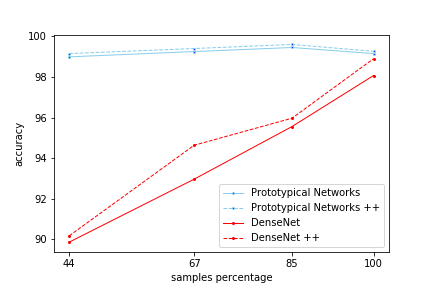
\includegraphics[width=0.32\columnwidth]{results/lsa16.png} \label{fig:results_varying_samples_lsa16}} & \subfigure[RWTH]{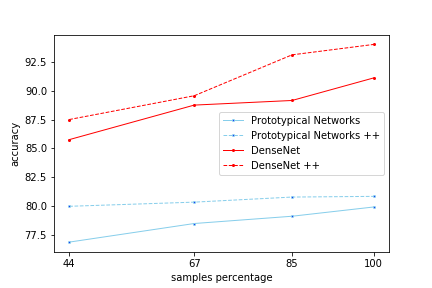
\includegraphics[width=0.32\columnwidth]{results/rwth.png} \label{fig:results_varying_samples_rwth}} & \subfigure[CIARP]{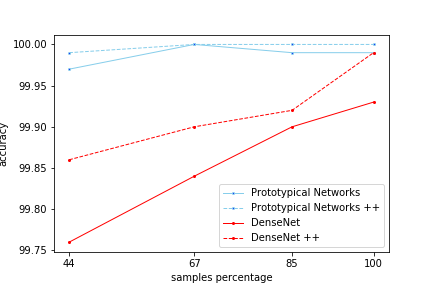
\includegraphics[width=0.32\columnwidth]{results/ciarp.png} \label{fig:results_varying_samples_ciarp}} \\
\end{tabular}
\caption{Accuracy of Prototypical Networks and DenseNet models trained by varying sample sizes on three datasets: LSA16, RWTH and CIARP. Each plot represents a different dataset where the x-axis is the percentage of samples used and the y-axis is the accuracy obtained. Models with "++" used data augmentation as described in this section. \label{fig:results_varying_samples}}
\end{figure}

\section{Conclusion}
\label{sec:conclusion}
We have performed experiments to evaluate the mean accuracy of Prototypical Networks and Wide-DenseNet on three handshape recognition datasets with and without data augmentation techniques.
For all datasets we found models that showed a performance on par  with or better than the state of the art.  Additionally, our results indicate that Wide-DenseNet benefits from data augmentation on all datasets except for CIARP.

 All models achieve near-perfect accuracy on CIARP.  This results show that  the dataset is too simple  as a benchmark for handshape recognition, seems while it has more samples on the other datasets (6000),  the samples are too  homogeneous and it does not have enough variation to generalize results to real-world application. Prototypical Networks  provide a new state-of-the-art accuracy on the LSA16  dataset,  surpassing all other known methods. Wide-DenseNets  also improve upon the state of the art,  and come close  to prototypical networks; by analyzing  the  variation of the accuracy  with respect to the training set size,  we can observe that  the performance gap between the two datasets  decreases sharply when the sample size increases.  We  have also obtained a new state-of-the-art on the RWTH  dataset  with Wide-DenseNet,  while Prototypical Networks also improved upon all previous results; this shows that  newer convolutional architectures can work better with  less data,  but there's still room for improvements using specialized models.

In future work, we  will focus on comparing with other datasets  to better understand the relationship between models and dataset complexities for handshape recognition.  We also see the need to compare with pre-trained models,  which are another way to alleviate the lack of data in a certain domain,  as well as methods that can  take advantage of unlabeled data.  Finally,  we will investigate the possibility of  merging data sets from different sign languages to augment the sample size,   as well as identify the types of data  augmentation that lead to  an improvement in state-of-the-art models.


\bibliographystyle{splncs03}
\bibliography{references,related}

\end{document}
